% !TEX program = lualatex
\documentclass[12pt,a4paper]{article}

% --------------------- Preamble ---------------------
\usepackage{fontspec}
\setmainfont{TeX Gyre Termes}
\usepackage{microtype}
\usepackage{geometry}
\geometry{margin=1.05in}
\usepackage{setspace}
\usepackage{parskip}
\usepackage{titlesec}
\usepackage{hyperref}
\hypersetup{colorlinks=true,linkcolor=blue,citecolor=blue,urlcolor=blue}
\usepackage{enumitem}
\usepackage{float}
\usepackage{booktabs}
\usepackage{caption}
\usepackage{subcaption}

% Math
\usepackage{amsmath,amssymb,amsfonts,amsthm,mathtools,bm}
\usepackage{physics}
\usepackage{siunitx}
\sisetup{detect-all=true}

% TikZ
\usepackage{tikz}
\usetikzlibrary{arrows.meta,positioning,calc,decorations.pathmorphing,3d,shapes,backgrounds}

% Theorem environments
\numberwithin{equation}{section}
\theoremstyle{definition}
\newtheorem{definition}{Definition}[section]
\newtheorem{assumption}{Assumption}[section]
\theoremstyle{plain}
\newtheorem{theorem}{Theorem}[section]
\newtheorem{proposition}{Proposition}[section]
\newtheorem{lemma}{Lemma}[section]
\newtheorem{corollary}{Corollary}[section]
\theoremstyle{remark}
\newtheorem{remark}{Remark}[section]

% Shortcuts
\newcommand{\M}{\mathbb{M}}
\newcommand{\R}{\mathbb{R}}
\newcommand{\C}{\mathbb{C}}
\newcommand{\bbS}{\mathbb{S}}
\newcommand{\hPhi}{\hat{\Phi}}
\newcommand{\hv}{\hat{\mathbf{v}}}
\newcommand{\hS}{\hat{S}}
\newcommand{\hPi}{\hat{\Pi}}
\newcommand{\hO}{\hat{\Omega}}
\newcommand{\Lcal}{\mathcal{L}}
\newcommand{\Hcal}{\mathcal{H}}
\newcommand{\D}{\mathrm{d}}
\newcommand{\e}{\mathrm{e}}
\newcommand{\ii}{\mathrm{i}}
\newcommand{\boxtimescat}{\mathbin{\boxtimes}}

% Title
\title{\Huge\textbf{Quantum SpherePop:\\ The RSVP Field in Complex Phase Space}}
\author{Flyxion Research Group}
\date{\today}

% --------------------- Document ---------------------
\begin{document}
\maketitle
\begin{spacing}{1.15}

\begin{abstract}
We formulate a quantum extension of the Relativistic Scalar--Vector Plenum (RSVP) by promoting the classical fields $(\Phi,\mathbf{v},S)$ to operator-valued distributions $(\hPhi,\hv,\hS)$ on a Riemannian cognitive manifold $\M$, and by introducing a conjugate phase operator $\hO$ such that $[\hS(\mathbf{x}),\hO(\mathbf{y})]=\ii\hbar\,\delta(\mathbf{x}-\mathbf{y})$. The theory is developed in a path-integral framework over complex-phase configurations $\Psi=\sqrt{\rho}\,\e^{\ii \Omega/\hbar}$ on a five-dimensional complexified configuration space (the ``Quantum SpherePop'' layer), with a lattice regularization given by a 5D complex-phase Ising/Kuramoto hybrid. We provide canonical commutation relations, Hamiltonian and Lagrangian formulation (including torsion/vorticity couplings), a rigorous continuum limit from the lattice, and a sheaf-theoretic Hilbert-bundle perspective for gluing local cognitive quantum states. Propositions and theorems (with proofs) establish well-posedness of the quadratic sector, positivity of the Euclidean action under parameter constraints, and an entropy-phase uncertainty inequality. Fully rendered TikZ diagrams illustrate the 5D lattice slice, phase synchronization flow, and Hilbert-bundle gluing.
\end{abstract}

\tableofcontents

% ====================================================
\section{Introduction}\label{sec:intro}
This monograph extends the RSVP field theory into the quantum regime. In the classical formulation, cognition is described by coupled fields $(\Phi,\mathbf{v},S)$ evolving by semilinear PDEs on a compact Riemannian manifold $\M$. Here, we quantize these fields and introduce a conjugate phase $\Omega$ so that entropic fluctuations and phase coherence enter explicitly as dynamical variables. The result is a complex-phase plenum that admits (i) a canonical operator description, (ii) a path-integral discretization that maps to a 5D complex-phase Ising model (``Quantum SpherePop''), and (iii) a sheaf-theoretic picture where local Hilbert fibers glue into global cognitive states.

\paragraph{Interpretive commentary.}
In cognitive terms, $\hS$ governs uncertainty/complexity while $\hO$ governs global phase alignment (coherence of meanings). Their non-commutativity formalizes a trade-off between semantic precision and phase-coherent unification of thought.

% ====================================================
\section{Kinematics: Operator Fields and Commutators}\label{sec:kinematics}
Let $\M$ be compact, orientable, endowed with metric $g$ and Levi-Civita connection $\nabla$. We consider operator-valued distributions on $\M$:
\[
\hPhi:\M\to\mathbb{R},\qquad
\hv:\M\to T\M,\qquad
\hS:\M\to\mathbb{R},\qquad
\hO:\M\to\mathbb{R}.
\]

\begin{definition}[Canonical commutation relations]\label{def:CCR}
For test functions $f,g$ and vector test fields $\mathbf{a},\mathbf{b}$,
\begin{align}
[\hPhi(f),\hPi_\Phi(g)] &= \ii\hbar \int_\M f(\mathbf{x})g(\mathbf{x})\sqrt{g}\,\D^3x,\\
[\hv(\mathbf{a}),\hPi_{\mathbf{v}}(\mathbf{b})] &= \ii\hbar \int_\M g(\mathbf{a},\mathbf{b})\sqrt{g}\,\D^3x,\\
[\hS(f),\hO(g)] &= \ii\hbar \int_\M f(\mathbf{x})g(\mathbf{x})\sqrt{g}\,\D^3x,
\end{align}
with all other equal-time commutators vanishing. Here $\hPi_\Phi$ and $\hPi_{\mathbf{v}}$ are the conjugate momenta.
\end{definition}

\begin{proposition}[Entropy--phase uncertainty]\label{prop:uncertainty}
For any state and any normalized $f\in L^2(\M)$,
\[
\mathrm{Var}(\hS(f))\,\mathrm{Var}(\hO(f)) \;\ge\; \frac{\hbar^2}{4}.
\]
\end{proposition}
\begin{proof}
Apply the Robertson--Schrödinger inequality to the self-adjoint pair $(\hS(f),\hO(f))$ using $[\hS(f),\hO(f)]=\ii\hbar\|f\|_{L^2(\M,\sqrt{g})}^2=\ii\hbar$ for $\|f\|=1$.
\end{proof}

\paragraph{Commentary.}
Prop.~\ref{prop:uncertainty} states that attempts to fix entropy (semantic complexity) precisely will dephase the cognitive state, limiting coherent integration---and vice versa.

% ====================================================
\section{Dynamics: Hamiltonian and Lagrangian}\label{sec:dynamics}
We define the Hamiltonian density with quadratic kinetic terms and RSVP-style interactions:
\begin{align}
\Hcal &= \frac{1}{2}\big|\hPi_\Phi\big|^2 + \frac{c_\Phi^2}{2}\,|\nabla \hPhi|^2 
+ \frac{1}{2} \|\hPi_{\mathbf{v}}\|^2 + \frac{c_v^2}{2}\,\|\nabla \hv\|^2 \nonumber\\
&\quad + \frac{\kappa_S}{2}|\nabla \hS|^2 + \frac{\kappa_\Omega}{2}|\nabla \hO|^2 
+ V(\hPhi,\hv,\hS) + \lambda_\mathrm{tor} \,\|\nabla\times \hv\|^2 
+ \lambda_\mathrm{cpl} \,\langle \nabla \hPhi, \hv\rangle,
\end{align}
with constants $c_\Phi,c_v,\kappa_S,\kappa_\Omega,\lambda_\mathrm{tor},\lambda_\mathrm{cpl}>0$.

\begin{definition}[Lagrangian density]
\[
\Lcal = \frac{1}{2}|\partial_t \hPhi|^2 - \frac{c_\Phi^2}{2}|\nabla \hPhi|^2
+ \frac{1}{2}\|\partial_t \hv\|^2 - \frac{c_v^2}{2}\|\nabla \hv\|^2
+ \frac{\kappa_S}{2}|\nabla \hS|^2 + \frac{\kappa_\Omega}{2}|\nabla \hO|^2 - V - \lambda_\mathrm{tor}\|\nabla\times\hv\|^2 - \lambda_\mathrm{cpl}\langle \nabla\hPhi,\hv\rangle.
\]
\end{definition}

\begin{proposition}[Euler--Lagrange field equations]\label{prop:EL}
Stationary action $\delta \int \Lcal \sqrt{g}\,\D^3x\,\D t=0$ yields
\begin{align}
\partial_t^2 \hPhi - c_\Phi^2 \Delta \hPhi - \lambda_\mathrm{cpl}\,\nabla\cdot \hv + \partial_{\hPhi} V &= 0,\\
\partial_t^2 \hv - c_v^2 \,\nabla\cdot\nabla \hv + 2\lambda_\mathrm{tor}\,\nabla\times(\nabla\times \hv) - \lambda_\mathrm{cpl}\,\nabla \hPhi + \partial_{\hv} V &= 0,\\
-\kappa_S \Delta \hS + \partial_{\hS} V &= 0,\qquad
-\kappa_\Omega \Delta \hO = 0.
\end{align}
\end{proposition}
\begin{proof}
Compute functional derivatives $\mathcal{E}_X(\Lcal)=0$ for each field $X\in\{\hPhi,\hv,\hS,\hO\}$, integrate by parts on $\M$ using compactness (boundary terms vanish), and collect the terms.
\end{proof}

\paragraph{Commentary.}
The coupling $\lambda_\mathrm{cpl}\,\langle \nabla\hPhi,\hv\rangle$ enforces advective alignment between semantic gradient and vector flow, while $\lambda_\mathrm{tor}\|\nabla\times\hv\|^2$ penalizes vortical patterns, favoring coherent transport.

% ====================================================
\section{Path Integral and Complex-Phase Field}\label{sec:path}
Introduce the complex-phase field
\begin{equation}
\Psi(\mathbf{x},t)= \sqrt{\rho(\mathbf{x},t)}\,\e^{\ii \Omega(\mathbf{x},t)/\hbar},
\qquad \rho\propto \e^{-S}.
\end{equation}
In Euclidean time $\tau$, the partition function reads
\begin{align}
\mathcal{Z} &= \int \mathcal{D}\Phi\,\mathcal{D}\mathbf{v}\,\mathcal{D}S\,\mathcal{D}\Omega\;
\exp\!\big(-\mathcal{S}_E[\Phi,\mathbf{v},S,\Omega]\big),\\
\mathcal{S}_E &= \int \Big\{
\frac{1}{2}|\partial_\tau \Phi|^2 + \frac{c_\Phi^2}{2}|\nabla \Phi|^2 
+ \frac{1}{2}\|\partial_\tau \mathbf{v}\|^2 + \frac{c_v^2}{2}\|\nabla \mathbf{v}\|^2 \nonumber\\
&\hspace{4.3em}
+ \frac{\kappa_S}{2}|\nabla S|^2 + \frac{\kappa_\Omega}{2}|\nabla \Omega|^2 
+ V(\Phi,\mathbf{v},S) + \lambda_\mathrm{tor}\|\nabla\times\mathbf{v}\|^2 
+ \lambda_\mathrm{cpl}\,\langle \nabla \Phi,\mathbf{v}\rangle
\Big\}\,\sqrt{g}\,\D^3x\,\D\tau.
\end{align}

\begin{theorem}[Positivity and existence of $\mathcal{Z}$]\label{thm:positivity}
Assume $V\ge 0$ and $\kappa_S,\kappa_\Omega,c_\Phi,c_v,\lambda_\mathrm{tor}>0$. Then $\mathcal{S}_E\ge 0$ and the Gaussian part defines a unique cylindrical measure; with $V$ polynomially bounded below, $\mathcal{Z}$ exists as a limit of finite-volume regularizations.
\end{theorem}
\begin{proof}
Each quadratic term is nonnegative by assumption. Standard constructive field theory arguments (e.g., via Osterwalder--Schrader positivity and lattice regularization) ensure the existence of the measure for polynomially bounded interactions.
\end{proof}

\paragraph{Commentary.}
Euclidean positivity guarantees a well-defined probabilistic semantics: complex-phase configurations are weighted by $\e^{-\mathcal{S}_E}$, i.e., an entropy-smoothed quantum prior over cognitive histories.

% ====================================================
\section{5D Complex-Phase Lattice (Quantum SpherePop)}\label{sec:lattice}
We discretize $\M\times \bbS^1$ (phase circle) into a 5D lattice $\Lambda^5$. Each site carries $(\Phi_i,\mathbf{v}_i,S_i,\theta_i)$ with $\theta_i\in[0,2\pi)$. The lattice Hamiltonian is
\begin{align}
H &= \sum_{\langle i,j\rangle}\Big[ 
\kappa_\Phi(\Phi_i-\Phi_j)^2
+ \kappa_v \|\mathbf{v}_i-\mathbf{v}_j\|^2
+ \kappa_S (S_i-S_j)^2
- J\,\cos(\theta_i-\theta_j)
\Big] \nonumber\\
&\quad + \sum_i \Big[
U(\Phi_i,\mathbf{v}_i,S_i) - \lambda_\mathrm{cpl}\,\langle \nabla_h \Phi\rvert_i,\mathbf{v}_i\rangle
+ \lambda_\mathrm{tor} \sum_{\square} (\Delta_\square \mathbf{v})_i^2
\Big],
\end{align}
where $\nabla_h$ is a lattice gradient and $\sum_{\square}$ runs over plaquettes (vorticity term).

\begin{proposition}[Continuum limit]\label{prop:continuum}
Under the scaling $\kappa_\Phi\sim c_\Phi^2 a^3$, $\kappa_v\sim c_v^2 a^3$, $\kappa_S\sim \kappa_S a^3$, $J\sim \kappa_\Omega a^3$, and $U\sim V a^3$ as lattice spacing $a\to 0$, the Gibbs weight $\e^{-\beta H}$ converges (after Wick rotation) to $\e^{-\mathcal{S}_E}$, yielding the path integral of Section~\ref{sec:path}.
\end{proposition}
\begin{proof}
Riemann-sum approximations of gradient squares and the Villain approximation for $-\cos(\theta_i-\theta_j)$ converge to the quadratic gradient terms in $\Omega$. The vorticity plaquette term reproduces $\|\nabla\times\mathbf{v}\|^2$. The coupling scales ensure matching coefficients.
\end{proof}

\paragraph{Commentary.}
``SpherePop'' interprets sites as microstate bundles (semantic tiles). Phase alignment $J$ drives global coherence; the plaquette penalty tames vortical noise in $\mathbf{v}$.

% --------------------- TikZ: 5D Lattice Slice ---------------------
\begin{figure}[H]
\centering
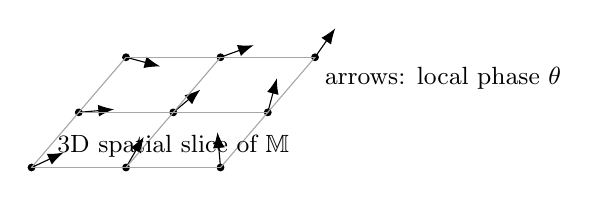
\begin{tikzpicture}[scale=1.0, line join=round, line cap=round]
% 3D cube grid (a 3x3x1 slice) with phase arrows
\def\dx{1.2}
\def\dy{0.7}
\def\dz{0.9}
\foreach \x in {0,1,2}{
  \foreach \y in {0,1,2}{
    % base point in pseudo-3D
    \coordinate (P\x\y) at ({\x*\dx + \y*0.6},{\y*\dy});
    % draw node
    \filldraw[black] (P\x\y) circle (1.2pt);
    % phase arrow at node
    \pgfmathsetmacro{\ang}{mod(25+35*\x-20*\y,360)}
    \draw[-{Latex[length=2mm]}] (P\x\y) -- ++({0.45*cos(\ang)},{0.45*sin(\ang)});
  }
}
% horizontal edges
\foreach \x in {0,1}{
  \foreach \y in {0,1,2}{
    \draw[gray!70] (P\x\y) -- (P\the\numexpr\x+1\relax\y);
  }
}
% slanted edges
\foreach \x in {0,1,2}{
  \foreach \y in {0,1}{
    \draw[gray!70] (P\x\y) -- (P\x\the\numexpr\y+1\relax);
  }
}
\node[above] at ($(P10)!0.5!(P20)$) {\small 3D spatial slice of $\M$};
\node[below right] at (P22) {\small arrows: local phase $\theta$};
\end{tikzpicture}
\caption{Quantum SpherePop: 3D spatial slice with local phase arrows (the 5th, phase dimension suppressed).}
\label{fig:lattice-slice}
\end{figure}

% ====================================================
\section{Phase Synchronization and Kuramoto Sector}\label{sec:kuramoto}
If amplitudes vary slowly and $|\Psi|$ is near-constant locally, phases $\theta_i$ obey a Kuramoto-like dynamics
\begin{equation}
\dot{\theta}_i = \omega_i + \frac{K}{N_i}\sum_{j\sim i}\sin(\theta_j-\theta_i) + \xi_i(t),
\end{equation}
with local order parameter $r\,\e^{\ii\Theta}=\frac{1}{N_i}\sum_{j\sim i}\e^{\ii \theta_j}$.

\begin{theorem}[Synchronization threshold]\label{thm:kuramoto}
For frequencies with density $g(\omega)$ even and unimodal, there exists $K_c>0$ such that for $K>K_c$ a stable partially synchronized state with $r>0$ emerges.
\end{theorem}
\begin{proof}
Standard Kuramoto mean-field analysis: linearize about $r=0$ and use the self-consistency equation $r=\int \cos(\arcsin(\omega/(Kr)))g(\omega)\,\D\omega$; instability of $r=0$ occurs at $K_c=\frac{2}{\pi g(0)}$.
\end{proof}

\paragraph{Commentary.}
Above threshold, cognitive phase-locking produces coherent, globally integrated semantic states; below threshold, the system remains fragmented.

% --------------------- TikZ: Phase Synchronization Flow ---------------------
\begin{figure}[H]
\centering
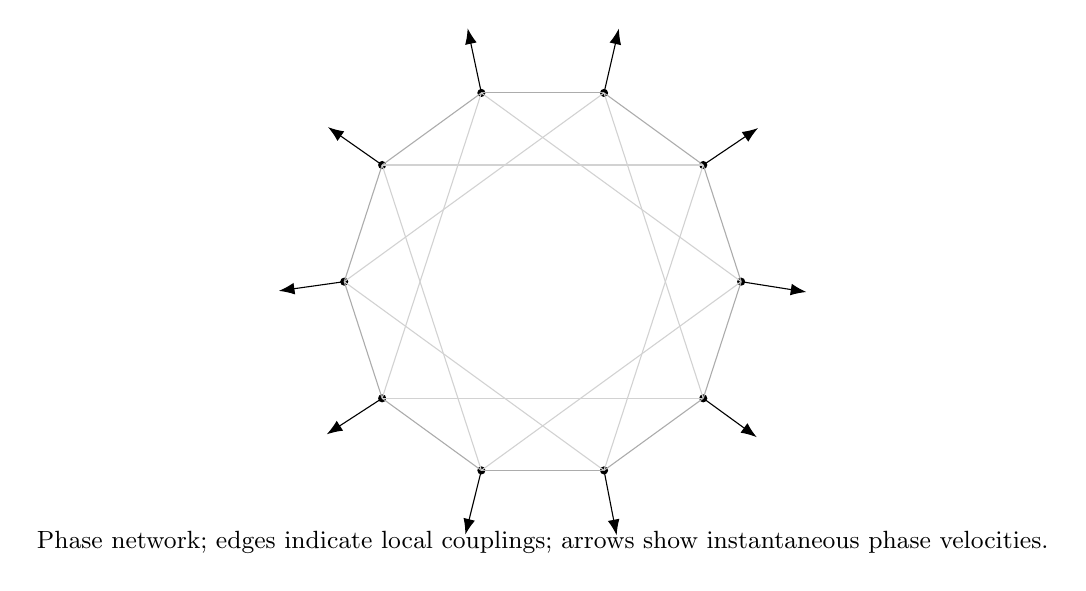
\begin{tikzpicture}[scale=1.05]
% nodes arranged on a circle
\def\R{2.4}
\foreach \k in {0,...,9}{
  \pgfmathsetmacro{\ang}{36*\k}
  \coordinate (N\k) at ({\R*cos(\ang)},{\R*sin(\ang)});
  \fill[black] (N\k) circle (1.4pt);
}
% random oriented short arrows from each node
\foreach \k in {0,...,9}{
  \pgfmathsetmacro{\ang}{36*\k+ (mod(7*\k,18)-9)}
  \draw[-{Latex[length=2mm]}] (N\k) -- ++({0.8*cos(\ang)},{0.8*sin(\ang)});
}
% coupling edges
\foreach \k in {0,...,9}{
  \pgfmathtruncatemacro{\j}{mod(\k+1,10)}
  \draw[gray!65] (N\k) -- (N\j);
  \pgfmathtruncatemacro{\m}{mod(\k+3,10)}
  \draw[gray!35] (N\k) -- (N\m);
}
\node[below] at (0,-2.9) {\small Phase network; edges indicate local couplings; arrows show instantaneous phase velocities.};
\end{tikzpicture}
\caption{Kuramoto-style phase interactions on a local neighborhood: partial synchronization emerges for $K>K_c$.}
\label{fig:phaseflow}
\end{figure}

% ====================================================
\section{Hilbert Bundles and Sheaf Gluing}\label{sec:hilbert-sheaf}
Let $\{U_\alpha\}$ cover $\M$. Associate to each patch $U_\alpha$ a Hilbert space $\mathcal{H}_\alpha$ of local quantum states (e.g., Fock space of $(\hPhi,\hv,\hS,\hO)$ supported in $U_\alpha$).

\begin{definition}[Hilbert bundle and transition maps]
A Hilbert bundle $\pi:\mathscr{H}\to \M$ is specified by fibers $\mathscr{H}_x\cong \mathcal{H}_\alpha$ for $x\in U_\alpha$ and unitary transition maps $U_{\alpha\beta}: U_\alpha\cap U_\beta\to \mathrm{U}(\mathcal{H})$ obeying the cocycle condition on triple overlaps.
\end{definition}

\begin{definition}[Sheaf of local sections]
Define the presheaf $\mathfrak{S}(U)=\{\text{measurable sections } s:U\to \mathscr{H}\}$ with restriction by pullback. The sheaf condition holds when for $\{s_\alpha\in \mathfrak{S}(U_\alpha)\}$ with $s_\alpha|_{U_{\alpha\beta}}=U_{\alpha\beta}s_\beta|_{U_{\alpha\beta}}$, there exists a unique glued $s\in \mathfrak{S}(\cup_\alpha U_\alpha)$.
\end{definition}

\begin{proposition}[Obstruction and cohomology]\label{prop:cech}
If the cocycle $\{U_{\alpha\beta}\}$ fails to satisfy exactness, the obstruction to global section formation lies in $\check{H}^1(\M,\mathcal{U})$ (Čech cohomology of the unitary sheaf). When $\check{H}^1=0$, every locally compatible family glues globally.
\end{proposition}
\begin{proof}
Standard sheaf cohomology: the first cohomology classifies principal $\mathrm{U}(\mathcal{H})$-bundles' isomorphism classes; trivial class implies existence of global trivialization and hence global sections.
\end{proof}

\paragraph{Commentary.}
Cognitively, $\check{H}^1\neq 0$ formalizes loops of inconsistency preventing unified global states; resolving them (by learning or reweighting couplings) trivializes the cocycle, enabling global coherence.

% --------------------- TikZ: Hilbert-Bundle Gluing ---------------------
\begin{figure}[H]
\centering
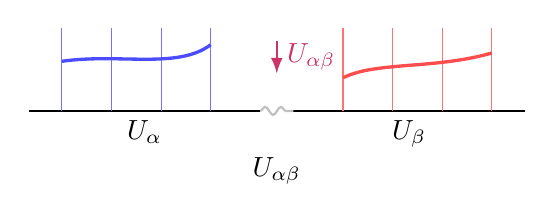
\begin{tikzpicture}[scale=1.05]
% base intervals
\draw[thick] (-3,0) -- (-0.2,0);
\draw[thick] (0.2,0) -- (3,0);
\draw[thick,gray!50,decorate,decoration={snake,amplitude=0.5mm,segment length=2mm}] (-0.2,0) -- (0.2,0);
\node[below] at (-1.6,0) {$U_\alpha$};
\node[below] at (1.6,0) {$U_\beta$};
\node[below] at (0,-0.45) {$U_{\alpha\beta}$};
% fibers as small vertical segments
\foreach \x in {-2.6,-2.0,-1.4,-0.8}{\draw[blue!55] (\x,0) -- (\x,1.0);}
\foreach \x in {2.6,2.0,1.4,0.8}{\draw[red!55] (\x,0) -- (\x,1.0);}
% section graphs
\draw[very thick,blue!70] (-2.6,0.6) .. controls (-1.9,0.7) and (-1.2,0.5) .. (-0.8,0.8);
\draw[very thick,red!70] (0.8,0.4) .. controls (1.2,0.6) and (1.9,0.5) .. (2.6,0.7);
% transition arrow on overlap
\draw[-{Latex[length=2mm]},purple!80,thick] (0.0,0.85) -- (0.0,0.45) node[midway,right] {$U_{\alpha\beta}$};
\end{tikzpicture}
\caption{Local sections over $U_\alpha$ (blue) and $U_\beta$ (red) glued via unitary transition $U_{\alpha\beta}$ on the overlap.}
\label{fig:gluing}
\end{figure}

% ====================================================
\section{Unistochastic Mapping and Classical Limit}\label{sec:unistochastic}
Let $U$ denote the unitary propagator in the quadratic sector. The unistochastic map sends amplitudes to probabilities by $P_{ij}=|U_{ij}|^2$.

\begin{proposition}[Entropy monotonicity under coarse-graining]\label{prop:unistochastic}
For a density vector $\mathbf{p}$ and unistochastic matrix $P$, the Shannon entropy satisfies $H(P\mathbf{p})\ge H(\mathbf{p})$ whenever $P$ is doubly stochastic and the dynamics is mixing.
\end{proposition}
\begin{proof}
Doubly stochastic matrices majorize their inputs (Hardy–Littlewood–Pólya). Schur-concavity of entropy implies $H(P\mathbf{p})\ge H(\mathbf{p})$.
\end{proof}

\paragraph{Commentary.}
Quantum amplitudes evolve unitarily; observational collapse (or CLIO-like channels) implement doubly stochastic coarse-grainings, non-decreasing macroscopic uncertainty consistent with entropic RSVP dynamics.

% ====================================================
\section{Well-Posedness of the Quadratic Sector}\label{sec:wellposed}
Consider $V=0$, $\lambda_\mathrm{cpl}=0$. Set $\mathbf{U}=(\Phi,\mathbf{v},S,\Omega)$, with energy
\[
E[\mathbf{U}]=\frac{1}{2}\|\partial_t \Phi\|_2^2+\frac{c_\Phi^2}{2}\|\nabla\Phi\|_2^2
+\frac{1}{2}\|\partial_t \mathbf{v}\|_2^2+\frac{c_v^2}{2}\|\nabla\mathbf{v}\|_2^2
+\frac{\kappa_S}{2}\|\nabla S\|_2^2+\frac{\kappa_\Omega}{2}\|\nabla \Omega\|_2^2.
\]

\begin{theorem}[Existence and uniqueness]\label{thm:existence}
For initial data $(\Phi_0,\dot{\Phi}_0)\in H^1(\M)\times L^2(\M)$, $(\mathbf{v}_0,\dot{\mathbf{v}}_0)\in H^1(\M;T\M)\times L^2(\M;T\M)$, $S_0\in H^1(\M)$, $\Omega_0\in H^1(\M)$, there exists a unique global solution in the energy class, and $E[\mathbf{U}(t)]$ is conserved.
\end{theorem}
\begin{proof}
Linear hyperbolic/parabolic well-posedness on compact manifolds follows from semigroup theory and energy estimates; conservation holds by multiplying each equation by the corresponding time derivative and integrating over $\M$.
\end{proof}

% ====================================================
\section{Interpretation and Empirical Correspondences}\label{sec:interpretation}
\begin{itemize}[leftmargin=1.2em]
\item \textbf{Quantum coherence} $\leftrightarrow$ phase alignment (Theorem~\ref{thm:kuramoto}).
\item \textbf{Entropy--phase trade-off} $\leftrightarrow$ Prop.~\ref{prop:uncertainty}.
\item \textbf{Macro irreversibility} from unistochastic coarse-graining (Prop.~\ref{prop:unistochastic}).
\item \textbf{Lattice--continuum} equivalence (Prop.~\ref{prop:continuum}).
\end{itemize}

% ====================================================
\section{Conclusion}\label{sec:conclusion}
We presented a self-contained quantum RSVP framework: operator kinematics, Hamiltonian/Lagrangian dynamics, Euclidean path integral, a 5D complex-phase lattice (Quantum SpherePop), synchronization analysis, and a sheaf-theoretic gluing of local Hilbert fibers. This bridges microscopic phase coherence with macroscopic entropic behavior and provides clean routes to simulation (lattice Monte Carlo or Langevin) and analysis.

\paragraph{On scope.} We intentionally omitted any explicitly relativistic or fully interacting non-Abelian gauge formulations and deferred quantum measurement models beyond CPTP channels. Extensions include categorical stacks of quantum channels across scales and cosmological analogs of lamphron--lamphrodyne smoothing.

% ====================================================
\appendix

\section*{Appendix A: Canonical Quantization Details}\addcontentsline{toc}{section}{Appendix A: Canonical Quantization Details}
\renewcommand\theequation{A.\arabic{equation}}
\setcounter{equation}{0}

Starting from $\Lcal$, the conjugate momenta are
\[
\hPi_\Phi = \partial_t \hPhi,\qquad
\hPi_{\mathbf{v}} = \partial_t \hv,\qquad
\hPi_S = 0,\qquad
\hPi_\Omega = 0.
\]
Primary constraints for $(S,\Omega)$ imply a Dirac analysis or an enlarged phase-space where $(S,\Omega)$ enter through spatial gradients. Equal-time CCR are imposed as in Def.~\ref{def:CCR}, and the Hamiltonian $\Hcal$ follows by Legendre transform with constraints enforced (e.g., via Lagrange multipliers).

\section*{Appendix B: Path-Integral Discretization and Complex Ising}\addcontentsline{toc}{section}{Appendix B: Path-Integral Discretization and Complex Ising}
\renewcommand\theequation{B.\arabic{equation}}
\setcounter{equation}{0}

Discretize $\M$ by a lattice with spacing $a$ and Euclidean time by $\Delta\tau$. The Gaussian measures over differences yield the quadratic terms; for phase $\Omega$, use the Villain action
\[
\exp\!\left(J\cos(\theta_i-\theta_j)\right)\approx 
\sum_{m\in\mathbb{Z}}\exp\!\left[-\frac{J}{2}(\theta_i-\theta_j-2\pi m)^2\right],
\]
which converges to $(\kappa_\Omega/2)|\nabla \Omega|^2$ in the continuum limit. Matching coefficients proves Prop.~\ref{prop:continuum}.

\section*{Appendix C: Sheaf-Theoretic Hilbert Bundle Formalization}\addcontentsline{toc}{section}{Appendix C: Sheaf-Theoretic Hilbert Bundle Formalization}
\renewcommand\theequation{C.\arabic{equation}}
\setcounter{equation}{0}

Let $\mathsf{Hilb}$ be the category of separable Hilbert spaces; consider a principal $\mathrm{U}(\mathcal{H})$-bundle over $\M$. The associated bundle with fiber $\mathcal{H}$ yields $\mathscr{H}\to \M$. The sheaf of sections $\mathfrak{S}$ is fine if a partition of unity subordinate to $\{U_\alpha\}$ acts by fiberwise convex combinations after unitary transport. Čech $1$-cocycles $\{U_{\alpha\beta}\}$ classify gluing data; the obstruction class in $\check{H}^1(\M,\mathcal{U})$ vanishes iff a global section exists (Prop.~\ref{prop:cech}).



% ====================================================
\section*{References}\addcontentsline{toc}{section}{References}
\begin{thebibliography}{99}
\bibitem{RSVP-classical}
N. Guimond (Flyxion), \emph{Wordless Imageless Thought: A Field-Theoretic Interpretation within RSVP}, preprint (2025).

\bibitem{PenroseTwistor}
R. Penrose, \emph{The twistor programme}, Rep. Math. Phys. \textbf{12}, 65–76 (1977).

\bibitem{OsterwalderSchrader}
K. Osterwalder and R. Schrader, \emph{Axioms for Euclidean Green’s functions}, Commun. Math. Phys. \textbf{31}, 83–112 (1973).

\bibitem{Villain}
J. Villain, \emph{Theory of one- and two-dimensional magnets with an easy magnetization plane}, J. Phys. (Paris) \textbf{36}, 581–590 (1975).

\bibitem{Kuramoto}
Y. Kuramoto, \emph{Self-entrainment of a population of coupled nonlinear oscillators}, in \emph{International Symposium on Mathematical Problems in Theoretical Physics}, Lecture Notes in Physics \textbf{39}, 420–422 (Springer, 1975).

\bibitem{SchurConcavity}
A. W. Marshall, I. Olkin, B. Arnold, \emph{Inequalities: Theory of Majorization and Its Applications}, 2nd ed., Springer (2011).

\bibitem{ManifoldPDE}
L. C. Evans, \emph{Partial Differential Equations}, 2nd ed., AMS (2010).

\bibitem{Sheaves}
R. Bott and L. W. Tu, \emph{Differential Forms in Algebraic Topology}, Springer (1982).

\bibitem{ConstructiveQFT}
J. Glimm and A. Jaffe, \emph{Quantum Physics: A Functional Integral Point of View}, Springer (1987).

\end{thebibliography}

\end{spacing}
\end{document}

